%%%%%%%%%%%%%%%%%%%%%%%%%%%%%%%%%%%%%%%%%%%%%%%%%%%%%%%%%%%%%%%%%%%%%%%%
%                                                                      %
%     File: Thesis_Background.tex                                      %
%     Tex Master: Thesis.tex                                           %
%                                                                      %
%     Author: Andre C. Marta                                           %
%     Last modified :  2 Jul 2015                                      %
%                                                                      %
%%%%%%%%%%%%%%%%%%%%%%%%%%%%%%%%%%%%%%%%%%%%%%%%%%%%%%%%%%%%%%%%%%%%%%%%

\chapter{Background}
\label{chapter:background}

This chapter presents some fundamental aspects necessary to the development of this dissertation.\par
First, a brief introduction to forging and its history followed by the forging processing steps, from the die design to the finishing processes.\par
Secondly, it is presented the additive manufacturing technology, as it appeared in this industry, which types of metallurgical processes are used and which new finishing processes developed are applied in \ac{AM} technology.\par
Finally, a brief theoretical review of the cost models that served as the basis for this dissertation.

\section{Forging Manufacturing}
\subsection{Forging Background}
\indent
As one of the oldest metallurgical processes, forging has a long history of development.\par
The first records of metalwork were discovered in the Middle East dated around 8000 BC. The formation of these metals was still rough, which limited their ability to work. \cite{navarro2006evoluccao} \par
The beginning of metallurgy coincides with the beginning of the age of metals around 4500/4000 BC. With the advancement of copper smelting around 4000 BC, it became a useful method to purify metals \cite{navarro2006evoluccao}. At this time, primitive men produced simple tools to assist in agriculture and to produce hunting weapons.\cite{azom}\par
The search for stronger materials led to the use of copper and tin alloys (Bronze Age) and later iron and carbon (Iron Age).\cite{navarro2006evoluccao} \par
Iron only appeared around 1200 BC, at the time to produce a piece of wrought iron, it was necessary to melt or heat it and then hammer it \cite{navarro2006evoluccao}. Hence forging was associated with a man who heated iron in the oven or on fire and with successive strokes of a hammer transformed the metal bar into a knife or sword, as seen in some Hollywood films about middle ages.\par
Most metallurgy items are made by hand until the 13th century. At this time, the tilting hammer, which used hydraulic energy, was developed. After lifting the hammer, the blacksmith dropped it and, under the force of gravity, it generated the forge blow. \cite{semiatin1988introduction}\par
The invention of steel by Bessemer,in the early 1856, it represented a great advance in this industry. Forgers were given a low-cost steel supplement to produce larger quantities of forgings. \cite{navarro2006evoluccao}
During the Industrial Revolution, at the end of the 18th century, with the increase of the production of ores such as steel and iron, there was a need for forging equipment that would allow the production of larger quantities of parts. This need was met with the development of the high speed steam hammer. This hammer produced several parts for firearms and parts for locomotives as well. \cite{semiatin1988introduction}\par
In the last 100 years, not only new types of machining equipment have been developed, but also new materials with special capabilities.\par
In 1930, the first forging press appeared. At the time with the appearance of motor vehicles by Henry Ford, the demand for forgings increased significantly, leading the National Machinery Company to invent Maxipress which increased the production rate and with a lesser degree of difficulty \cite{azom}.\par
The emergence of electrical power and technological advances,  computer-controlled hammers and presses are capable of making a wide range of components in a variety of materials for many applications, including aerospace, automotive, mining and agriculture, among others.\par
Recently, the automotive and aerospace industries account for about 50\% of US production using forge techniques \cite{site2}, as we can see in figure 2.1.

\begin{figure}[h]
\centering
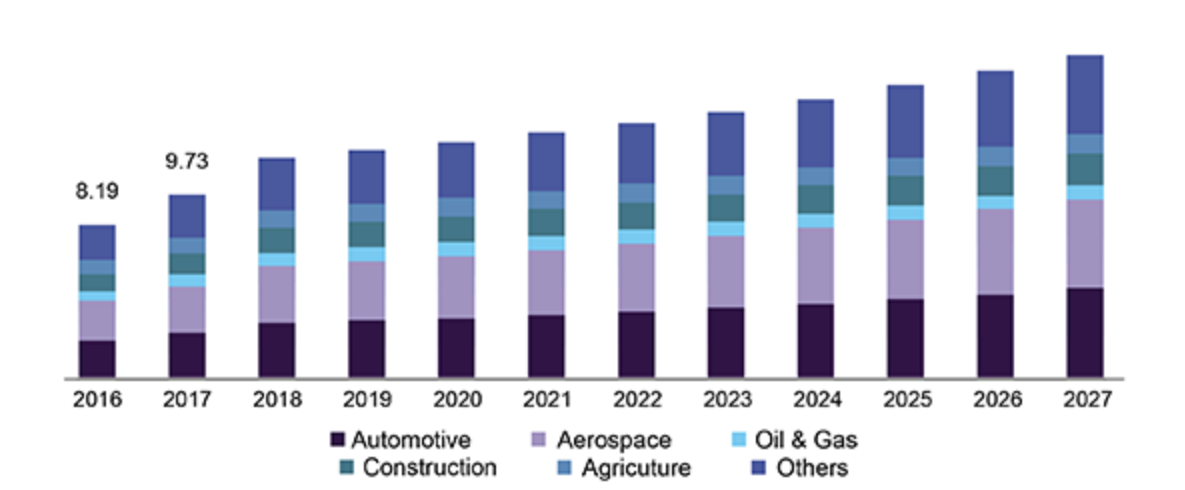
\includegraphics[width=0.6\textwidth]{./Images/Forgingindustry.png}
\caption{U.S. metal forging market size, 2016-2027 (USD Billion)}
\label{ForgingMarket}
\caption*{\textbf{Source}: www.grandviewresearch.com}
\end{figure}

Globally, the commercial segment represents around 51 \% of the aerospace industry in the United States, figure \ref{Forg2}, due to the fact that the demand for air passengers for Asia-Pacific travel is increasing over time. The second is the military segment, which is estimated to grow due to the increase of the defense budget, which remains one of the flags of this country\cite{market}.\par
Nowadays, the automotive and aerospace industries account for about 50\% of US production using forging techniques \footnote[]{These predictions were made before and during the appearance of the COVID-19 virus. Since the aerospace industry was one of the sectors most affected, they may not be up to date.\cite{hall2020beyond}},as we can see in figure \ref{ForgingMarket} \cite{market}.\par




\begin{figure}[h]
\centering
\includegraphics[width=0.6\textwidth]{./Images/Forg2.png}
\caption{Global aerospace forging market share, by aircraft, 2019 (\%)}
\label{Forg2}
\caption*{\textbf{Source}: www.grandviewresearch.com}
\end{figure}




\subsection{Forging Process}

Forging is a process that converts a metal in an object through compressive forces on a discrete part in a set of dies.
The process requires a few steps which depend on the complexity of the object to be produced.
Figure \ref{ForgingSteps1} is shown the generalized stages of typical forging process.

\begin{figure}[h]
\centering
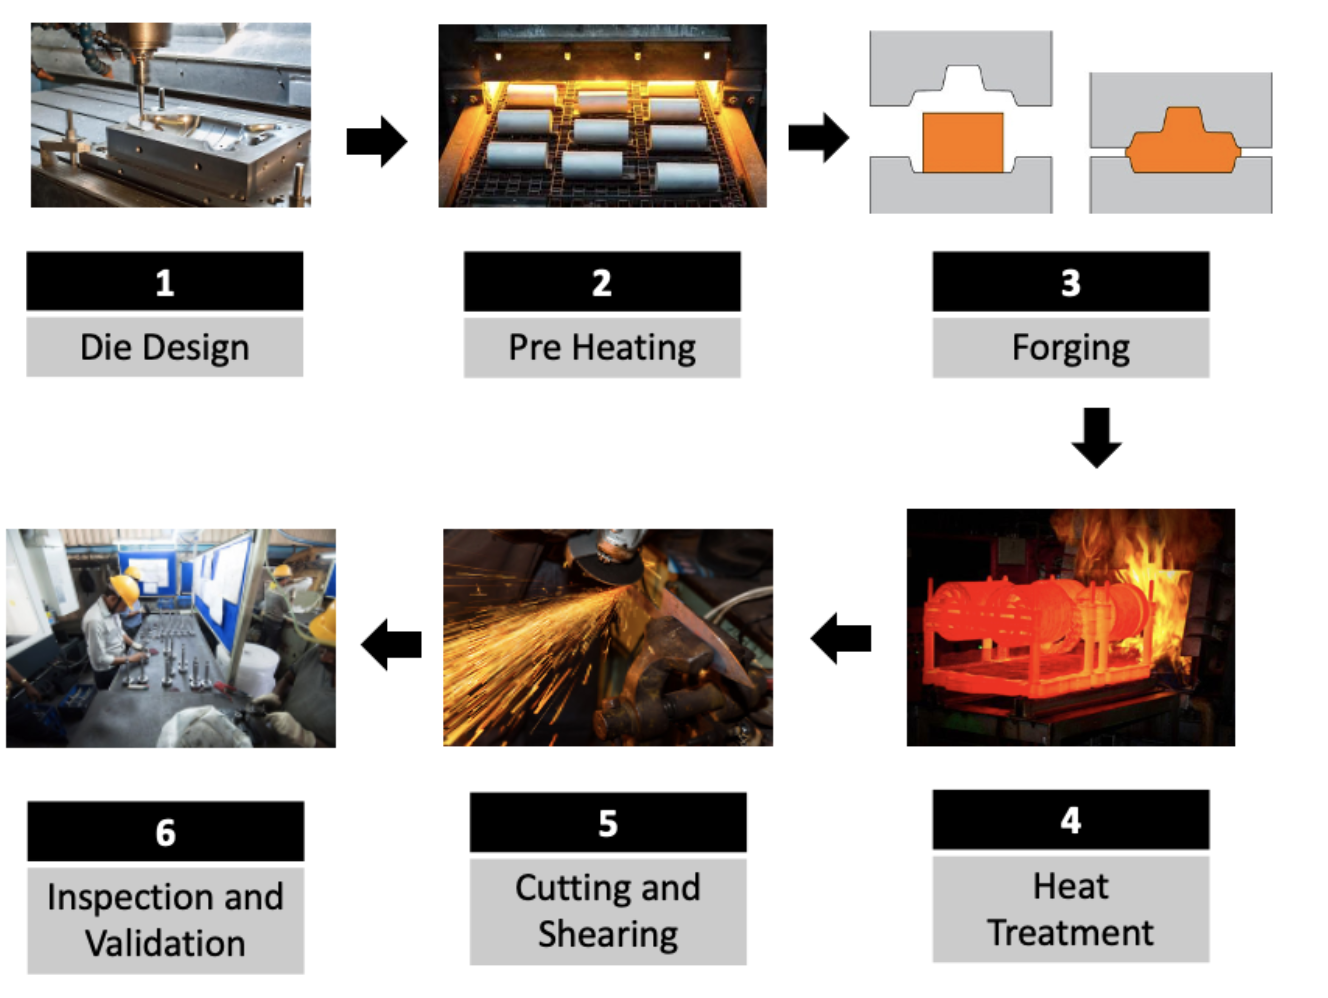
\includegraphics[width=0.7\textwidth]{./Images/ForgingSteps.png}
\caption{Generalized Forging Process}
\label{ForgingSteps1}
\end{figure}

\textbf{\emph{1. Die Design and Design of Forging Parameters}}\\

Die and mold manufacturing represents a significant area of production technology , the most restrictive aspect to be considered is the tools' cost. The construction of a metal stamping die requires a high number of resources and people, which will make the die building more expensive and, for this reason the bigger quantity of parts produced the more economically profitable it becomes \cite{souza2015estudo}.\par
The manufacture of a die and its ability to produce parts depends on several factors. The main areas of concern are:
\begin{itemize}
    \item \textbf{Parting Line} - The Parting Line is usually the central line, which separates the two dies. For a complex part, designing the parting line may not be a simple task \cite{site3,smith1990design}.
    \item \textbf{Flash and Gutter} - During the compression of the material against the die, the flash material can flow into a gutter. A good design can prevent an unnecessary increase of the forging load with excess flash \cite{site3,smith1990design}.
    \item \textbf{Draft Angles} - When designing the die, it is necessary to take into account the way the part will be removed from the die. Tilt angles are sometimes used to facilitate this removal \cite{site3,smith1990design}.
    \item \textbf{Fillet} - The fillet is a small radius provided at the corners to ensure smooth flow of metal into the matrix cavity. A small fillet leads to rapid wear of the die and an improper metal slip \cite{site3,smith1990design}.
    \item \textbf{Die material} - 
The die must be made of a hard material resistant not only to high temperatures but also resistant to mechanical and thermal shocks, as well as it should be a high resistance to wear \cite{site3,smith1990design}.
\end{itemize}



\vspace{50}


\textbf{ \emph{2. Pre Heating}}\\

Depending on the temperature at which the metal is forged, the forging can be classified as cold, warm or hot forging.\par
Cold forging involves forging with open die or close die and use of lubricant close to room temperature. Forgings of carbon steel and standard alloys are commonly cold forged, not requiring this production step. This type of forging offers an economically competitive advantage, since the forged part requires little finishing that normally makes the part more expensive\cite{site5,bryson2005heat}.\par
Warm forging is a type of forging that forges the part above the ambient temperature to below the recristallization temperature. Compared to cold forging, warm forging has the potential advantages of reduced tool loads, increased ductility, elimination of annealing needing before forging and favorable forging properties that can eliminate heat treatment\cite{site5,bryson2005heat}.\par
In hot forging, the metal and the die are heated to the same temperature. The objective of this step is to avoid hardening by deformation, in this way the metal is heated to the recrystallization temperature in such a way that the recrystallization occurs simultaneously with the plastic deformation\cite{site5,bryson2005heat}.\par
Hot forged components have greater ductility, which makes them desirable for many configurations. In addition, as a technique, hot forging is more flexible than cold forging, as customized parts can be manufactured\cite{site5,bryson2005heat}. \par
\vspace{5}


\textbf{\emph{2. Forging}}\\

During forging the metal is compressed under high pressure for a part to reach the desired shape. \par
In general, forging can be classified based on how metal flow is confined, as open die or closed die[14], figure \ref{OpenClosedDied}. \par


\begin{figure}[h]
  \centering
  \begin{minipage}[b]{0.4\textwidth}
    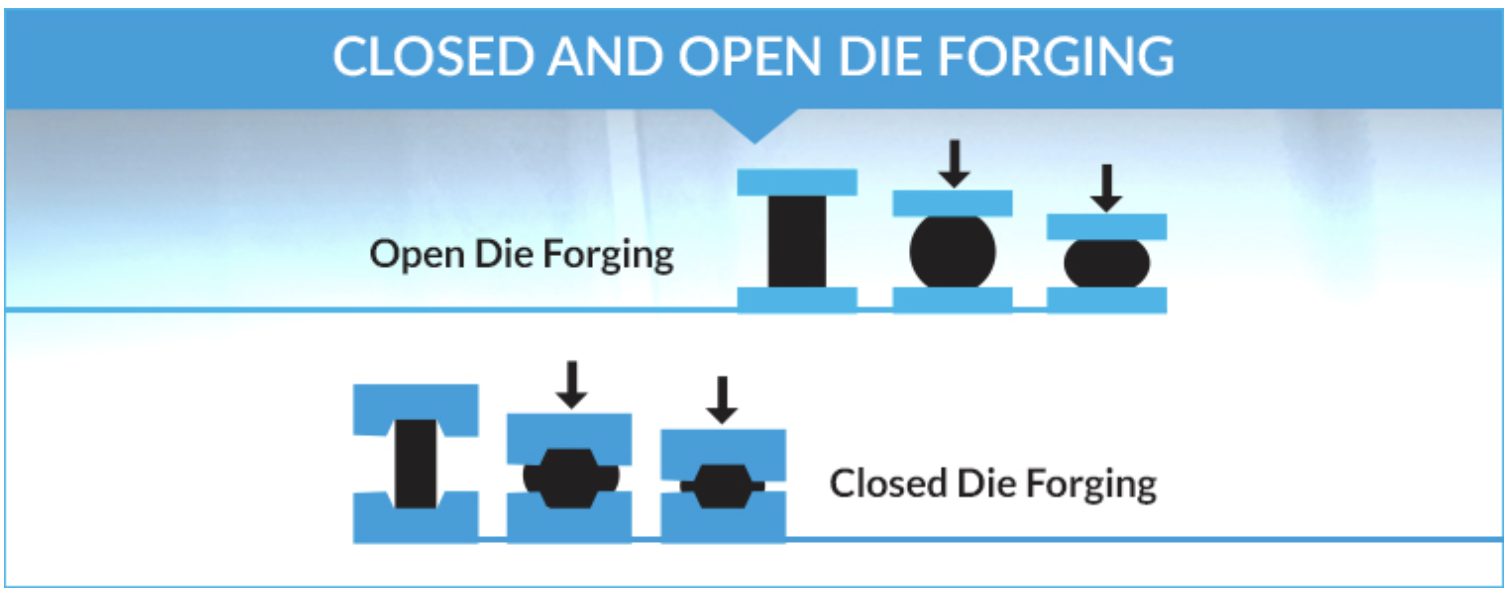
\includegraphics[width=\textwidth]{./Images/closedopen_die.png}
    \caption{Closed and Open Die Forging}
    \label{OpenClosedDied}
    \caption*{\textbf{Source:}www.indiaforging.com}
  \end{minipage}
  \hfill
  \begin{minipage}[b]{0.4\textwidth}
    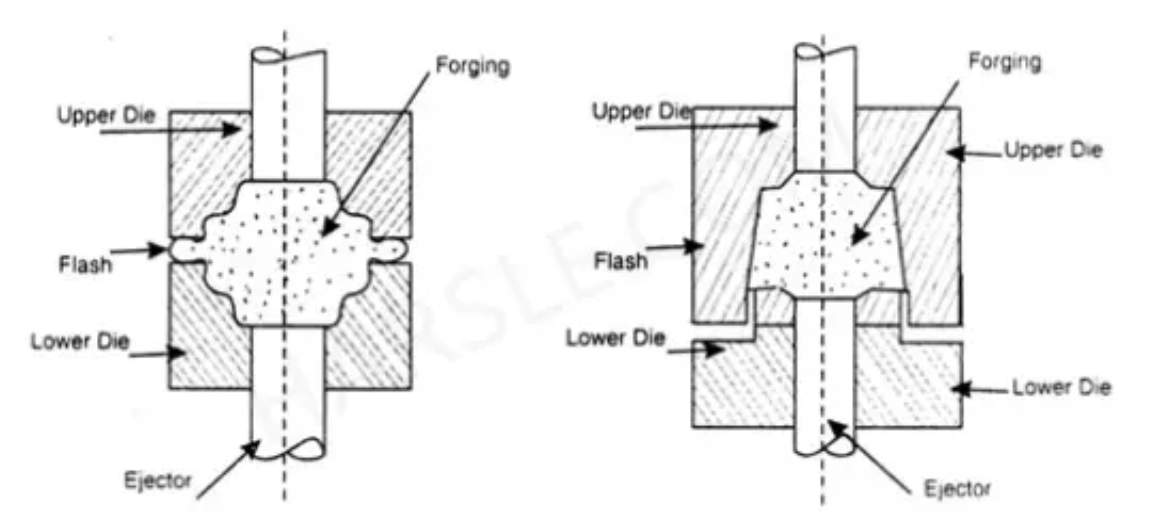
\includegraphics[width=\textwidth]{./Images/Flashless_die.png}
    \caption{Flash and Flashless Hot Forging}
    \label{Flashforging}
    \caption*{\textbf{Source:}www.harsle.com}
  \end{minipage}
\end{figure}

Forging is the molding of metal by plastic deformation. This process covers a multitude of equipment and techniques.
We can classify forging by:
\begin{itemize}
    \item Forging temperature - Hot, Warm or Cold Forging
    \item Die shape - Open Die Forging or Close Die Dorging
    \item Compressive forces - Drop Forging, Press Forging or Rolling Forging
\end{itemize}

Regarding the temperature and the type of die, it has been analyzed previously.\par
A far as of the shape of the die is concerned, forging can be classified as open die forging or close die forging.\par
Open die forging is performed using two flat dies, which are not normally touched, or which allows the material to be released freely in the lateral direction. This type of forging is used for large parts or discs, blocks or bars.\cite{site4,site3,souza2015estudo}\par
In closed die forging or  impression-die, the cavity is formed by using two or more dies which the metal is deforming undergoes plastic deformation through the pressure exerted \cite{site4} \cite{site3,souza2015estudo}.\par
Forging is a method of handling the metal to achieve the final product. Usually the design of this product is in a die, where the metal is pressed against it to obtain the desired shape. This metal manipulation is usually done using two methods: Drop forging or press forging. \par
A closed die can also be selected as flash or flashless, \textif{c.f.} figure \ref{Flashforging}. The flashless forging allows excess material not to escape through the concavity, while the flash type can occur \cite{site4,site3,souza2015estudo}.\par
The advantage of this forging is that it allows more complex shapes and closer tolerances than forging in the open die. Limit your ability to produce parts in great detail, or forging prevalent in the metallurgical industry\cite{site5,souza2015estudo}.\par

In the Drop Forging, forge hammers are used to deform the metal through several impact strikes on the metal surface \cite{site3,altan2004cold}. During the process the surface layers of the metal are manipulated in shape. However, the central area of the metal will remain relatively deformed. In this process, the deformation rate is difficult to control and generally the cost of this product is generally lower, for low production volumes, when compared to press forging \cite{site3,altan2004cold}.  \pair

In the press forging a slower and continuous pressure speed is used. The material is shaped evenly, from the surface to the center, making it an advantage over drop forging, as it allows for a stronger and more perfect final product\cite{site3,altan2004cold}.  \pair
In this process, the initial costs are much higher than using a hammer, making it more economical with increasing production volume. Despite being a longer technique, another advantage is a more controlled deformation rate that allows a stronger product\cite{site3,altan2004cold}. \par

Roll forging consists of two horizontal cylindrical rollers that form a round or flat bar. This type of forging is used to increase the length or decrease the thickness of the metal bar. This bar is heated and then passed through two rollers that contain patterned grooves and is progressively shaped as it is rolled by the machine \cite{site3}.\par
\vspace{20}
\textbf{ \emph{3. Heat Treatment}}\\

Heat treatment can be defined as controlled heating or cooling of metals made with a change in physical and mechanical properties.\par
In many cases, as metal parts go through different temperatures during a heating phase, going through heating and cooling cycles, thus altering some physical and mechanical characteristics of parts, with the possibility of having thermally affected parts zones \cite{bryson2005heat,souza2015estudo}. \par
However, heat treatment can be used for different purposes: to increase the material's resistance and/or to decrease the excess duration, allowing better machining and restoring ductility after an intense cold machining process \cite{bryson2005heat,souza2015estudo}. \par
The figure \ref{HTsteps}, it helps to understand how the heat treatment takes place.

\begin{figure}[h]
\centering
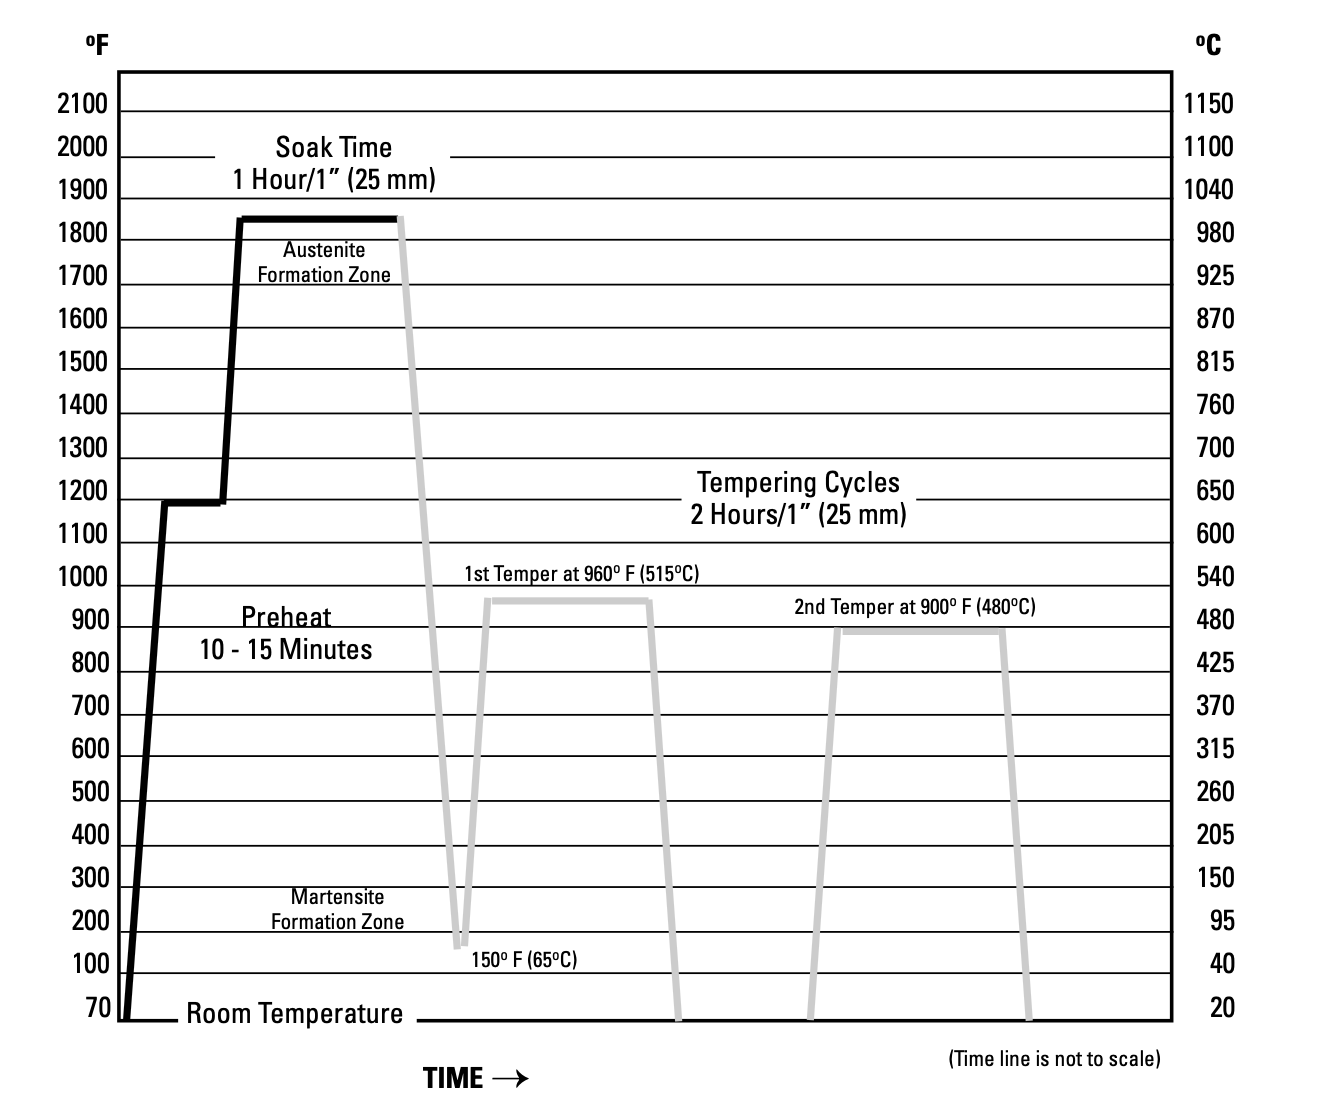
\includegraphics[width=0.6\textwidth]{./Images/HotTreat.png}
\caption{Generalized Hot Treatment Steps}
\label{HTsteps}
\caption*{\textbf{Source:} Heat treatment, selection, and application of tool steels \cite{bryson2005heat}}
\end{figure}

Depending on the application of the forged part, the residence times in the oven and the temperature at which the part must be raised are defined.
The main heat treatments used in forged metals are Annealing, Normalization, Stress Relief, Queching and Tempering.

\emph{Complete annealing} is a very general term that consists of heating the part above the critical zone and letting it cool slowly. Annealing will produce a more refined microstructure, in order to soften the metal to better withstand the constant pressures that the metal may undergo during the machining process \cite{huang2006hardening}. For this reason, this heat treatment is often used not only as a finishing process but also as a preheat use before machining. \cite{bryson2005heat,souza2015estudo}

\emph{Normalization} is a technique used to offer uniformity in grain size to the piece's metal. When normalized, the piece is heated to a temperature just above the critical point, keeping enough time to form smaller and more uniform metal grains. After heating above the critical point, the part is cooled in the open air until it reaches room temperature.
 This transformation is called grain refinement, which takes the piece to become more uniform, but above all improving the strength and toughness of the material.\cite{bryson2005heat,souza2015estudo}
 
\emph{Stress relief} is a technique for removing internal stress from a metal. These stresses can be caused many times by the process of cold machining or non-uniform cooling. Stress relief consists of reheating the metal below the critical temperature and then uniformly cooling the part.\cite{bryson2005heat}

\emph{Quenching} involves rapidly cooling the material after heating it above the critical region. After being quickly cooled, the alloy turns into martensite, a hard and brittle crystalline structure. For this reason, after Quenching, tempering is normally used.\cite{bryson2005heat,souza2015estudo}
\emph{Tempering}
Martensite steel is very hard but very brittle. Tempering is the heat treatment that seeks to offer a better combination of hardness, strength and toughness.
Tempering is effective in relieving tensions caused by cooling, in addition to decreasing hardness for specific intervals.\cite{bryson2005heat,souza2015estudo}
In this process, the metal is reheated to a relatively low temperature with a controlled time to produce the desired final requirements for the part.

\vspace{50}

\textbf{ \emph{4. Cutting and Shearing}}\\


\textbf{\emph{Wire Electric Discharge Machining}}\par 
\vspace{5}\par
Wire \ac{EDM} is a machining process that emerged in the 1960s with the aim of manufacturing hardened steel die \cite{el2018fundamentals}. It is a non-traditional machining process widely used in today's manufacturing. It involves removing metal using an electric discharge wire machining the part with high speed and accuracy \cite{tominaga1987electrode,rajurkar2013review}.\par 
This relatively recent technology is commonly used for machining hard materials that are difficult to work with conventional forging. The process consists of immersing a part in a dielectric which use a cutting wire powered electrically that cuts the metal, \textif{c.f.} figure \ref{EDM} \cite{rajurkar2013review}. First, machines used a \ac{NC} and nowadays they use \ac{CNC}. \par
This technology has brought several benefits, since it allows the cutting of very hard materials without them being subjected to excessive pressure from the impact used in machining. It also allows achieving high design tolerances \cite{el2018fundamentals}.\par

\vspace{10}

\textbf{\emph{Multi Axis Mills}}
\vspace{5}\par
\ac{MM} is a process that involves a tool that moves in 3, 4 or 5 directions depending on the type of machine. This machine,\textit{c.f.} figure \ref{MM}, allows the milling of excess material with a water jet or laser cut \cite{el2018fundamentals}.\par
In the most recent machines, a CAD is used through computer software that will allow the machine to know where to cut. This technology allows a better finish of the piece for more complex pieces, and the detail of them can be increased \cite{son2009hybrid}.\par
Since the machines are using a software witch give a precise indications of cutting the part, then this can be replicated hundreds of times and each product will be exactly the same, in addition to needing only a supervision of it.\par
\vspace{5}


\begin{figure}[h]
  \centering
  \begin{minipage}[b]{0.45\textwidth}
    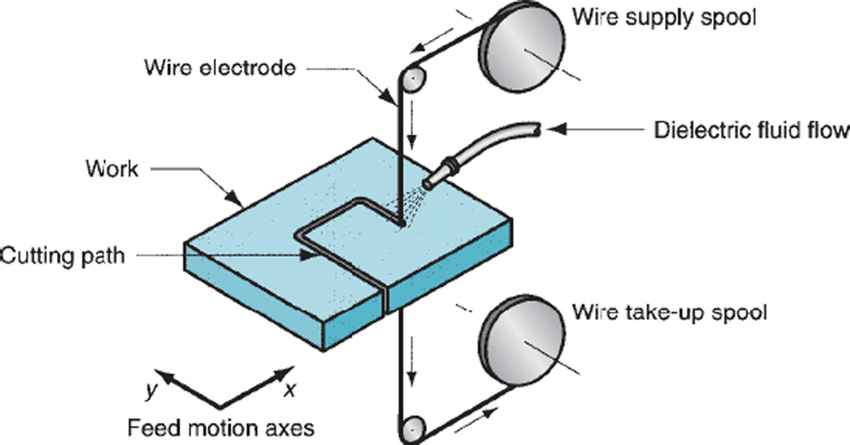
\includegraphics[width=\textwidth]{./Images/EDM.png}
    \caption{EDM Cutting Process}
    \label{EDM}
    \caption*{\textbf{Source:} Comprehensive materials finishing \cite{saleh20171} }
  \end{minipage}
  \hfill
  \begin{minipage}[b]{0.3\textwidth}
    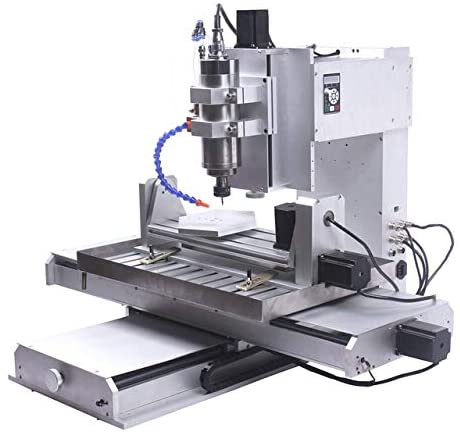
\includegraphics[width=\textwidth]{./Images/MM.png}
    \caption{A 5-axis Multi Axis Machine and a part manufactured with it.}
    \label{MM}
    \caption*{\textbf{Source:} www.wardjet.com}
  \end{minipage}
\end{figure}

\vspace{10}
\textbf{\emph{Thermochemical Treatment}}\par
\vspace{10}
This treatment aims to change the surface properties of the metal. In general, materials with high hardness have a high resistance to wear, but low toughness and resistance to impact.\par
In some parts, a tough core and a wear-resistant surface are desired. For this reason, low carbon steels are subjected to thermochemical treatment by carburizing, which increases the carbon content on the surface, increasing its resistance to wear, while preserving the properties of the core.The means to carry out the treatment are carbon or nitrogen sources which can be in the form of solids, liquids or gases \cite{czerwinski2012thermochemical}.\par
The process consists of combining repeated heating and cooling, keeping the material in contact with C or N, such as specific salts, oils or gases for that purpose \cite{czerwinski2012thermochemical}.\par
\vspace{5}
\textbf{\emph{Grinder}}
\vspace{5}

Grinding is an important metal machining process. The process allows for a finer finish and increases the useful life of the part \cite{el2018fundamentals,malkin1984grinding}.
With the interaction of abrasive grains on the surface of the part, metal removal occurs \ref{grinder2}. This removal occurs by a shearing process in which it normally involves a rotating wheel with abrasive particles on the metal surface, firgure \textit{c.f.} \ref{grinder1} \cite{el2018fundamentals,malkin1984grinding}. Several machines are used in this process as:
\begin{itemize}
    \item Whetstone;
    \item Power tools such as angle grinders;
    \item Bench grinders.
\end{itemize}

The process today can be used through an axis machine, such as Multi Axis Mills, in which it uses \ac{CNC}.

\begin{figure}[h]
  \centering
  \begin{minipage}[b]{0.4\textwidth}
    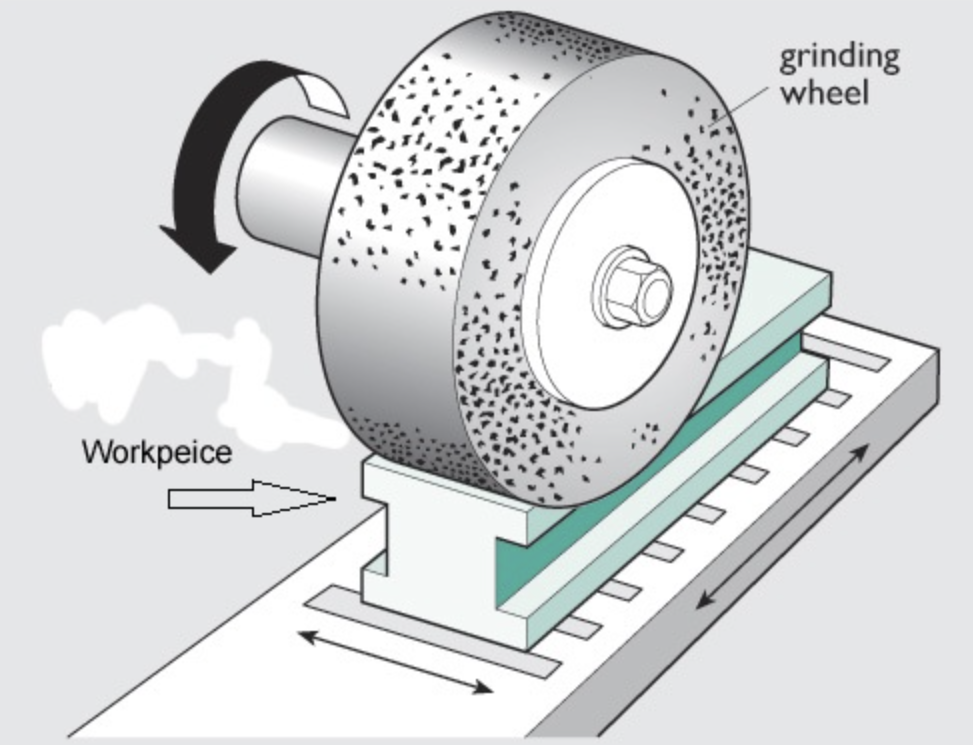
\includegraphics[width=\textwidth]{./Images/GW.png}
    \caption{Grinder Rotating Wheel}
    \label{grinder1}
    \caption*{\textbf{Source:} www.surfacegrindingmachine.wordpress.com}
  \end{minipage}
  \hfill
  \begin{minipage}[b]{0.45\textwidth}
    
\includegraphics[width=\textwidth]{./Images/grinder2.png}
    \caption{Abrasive Process in Grinder}
    \label{grinder2}
    \caption*{\textbf{Source:} www.wikipedia.org/grinder}
  \end{minipage}
\end{figure}



\pagebreak

% #############################################################################
\section{AM Technology}

\subsection{Introduction}
Additive Manufacturing, also called 3D Printing, is a relatively recent method of manufacturing parts from \ac{CAD} file. In contrast to subtractive manufacturing methods, such as forging, AM generally builds the part layer by layer.\par
A computer-developed project is exported to the \ac{STL} file format that is read by the equipment AM that build it. \par
Nowadays, AM can produce parts using any type of raw material, from plastics, metals, ceramics to composites. There are several techniques available that can be classified according to their raw material: powder base, liquid base and solid base.\\

\subsection{History}

\begin{figure}[h]
\centering
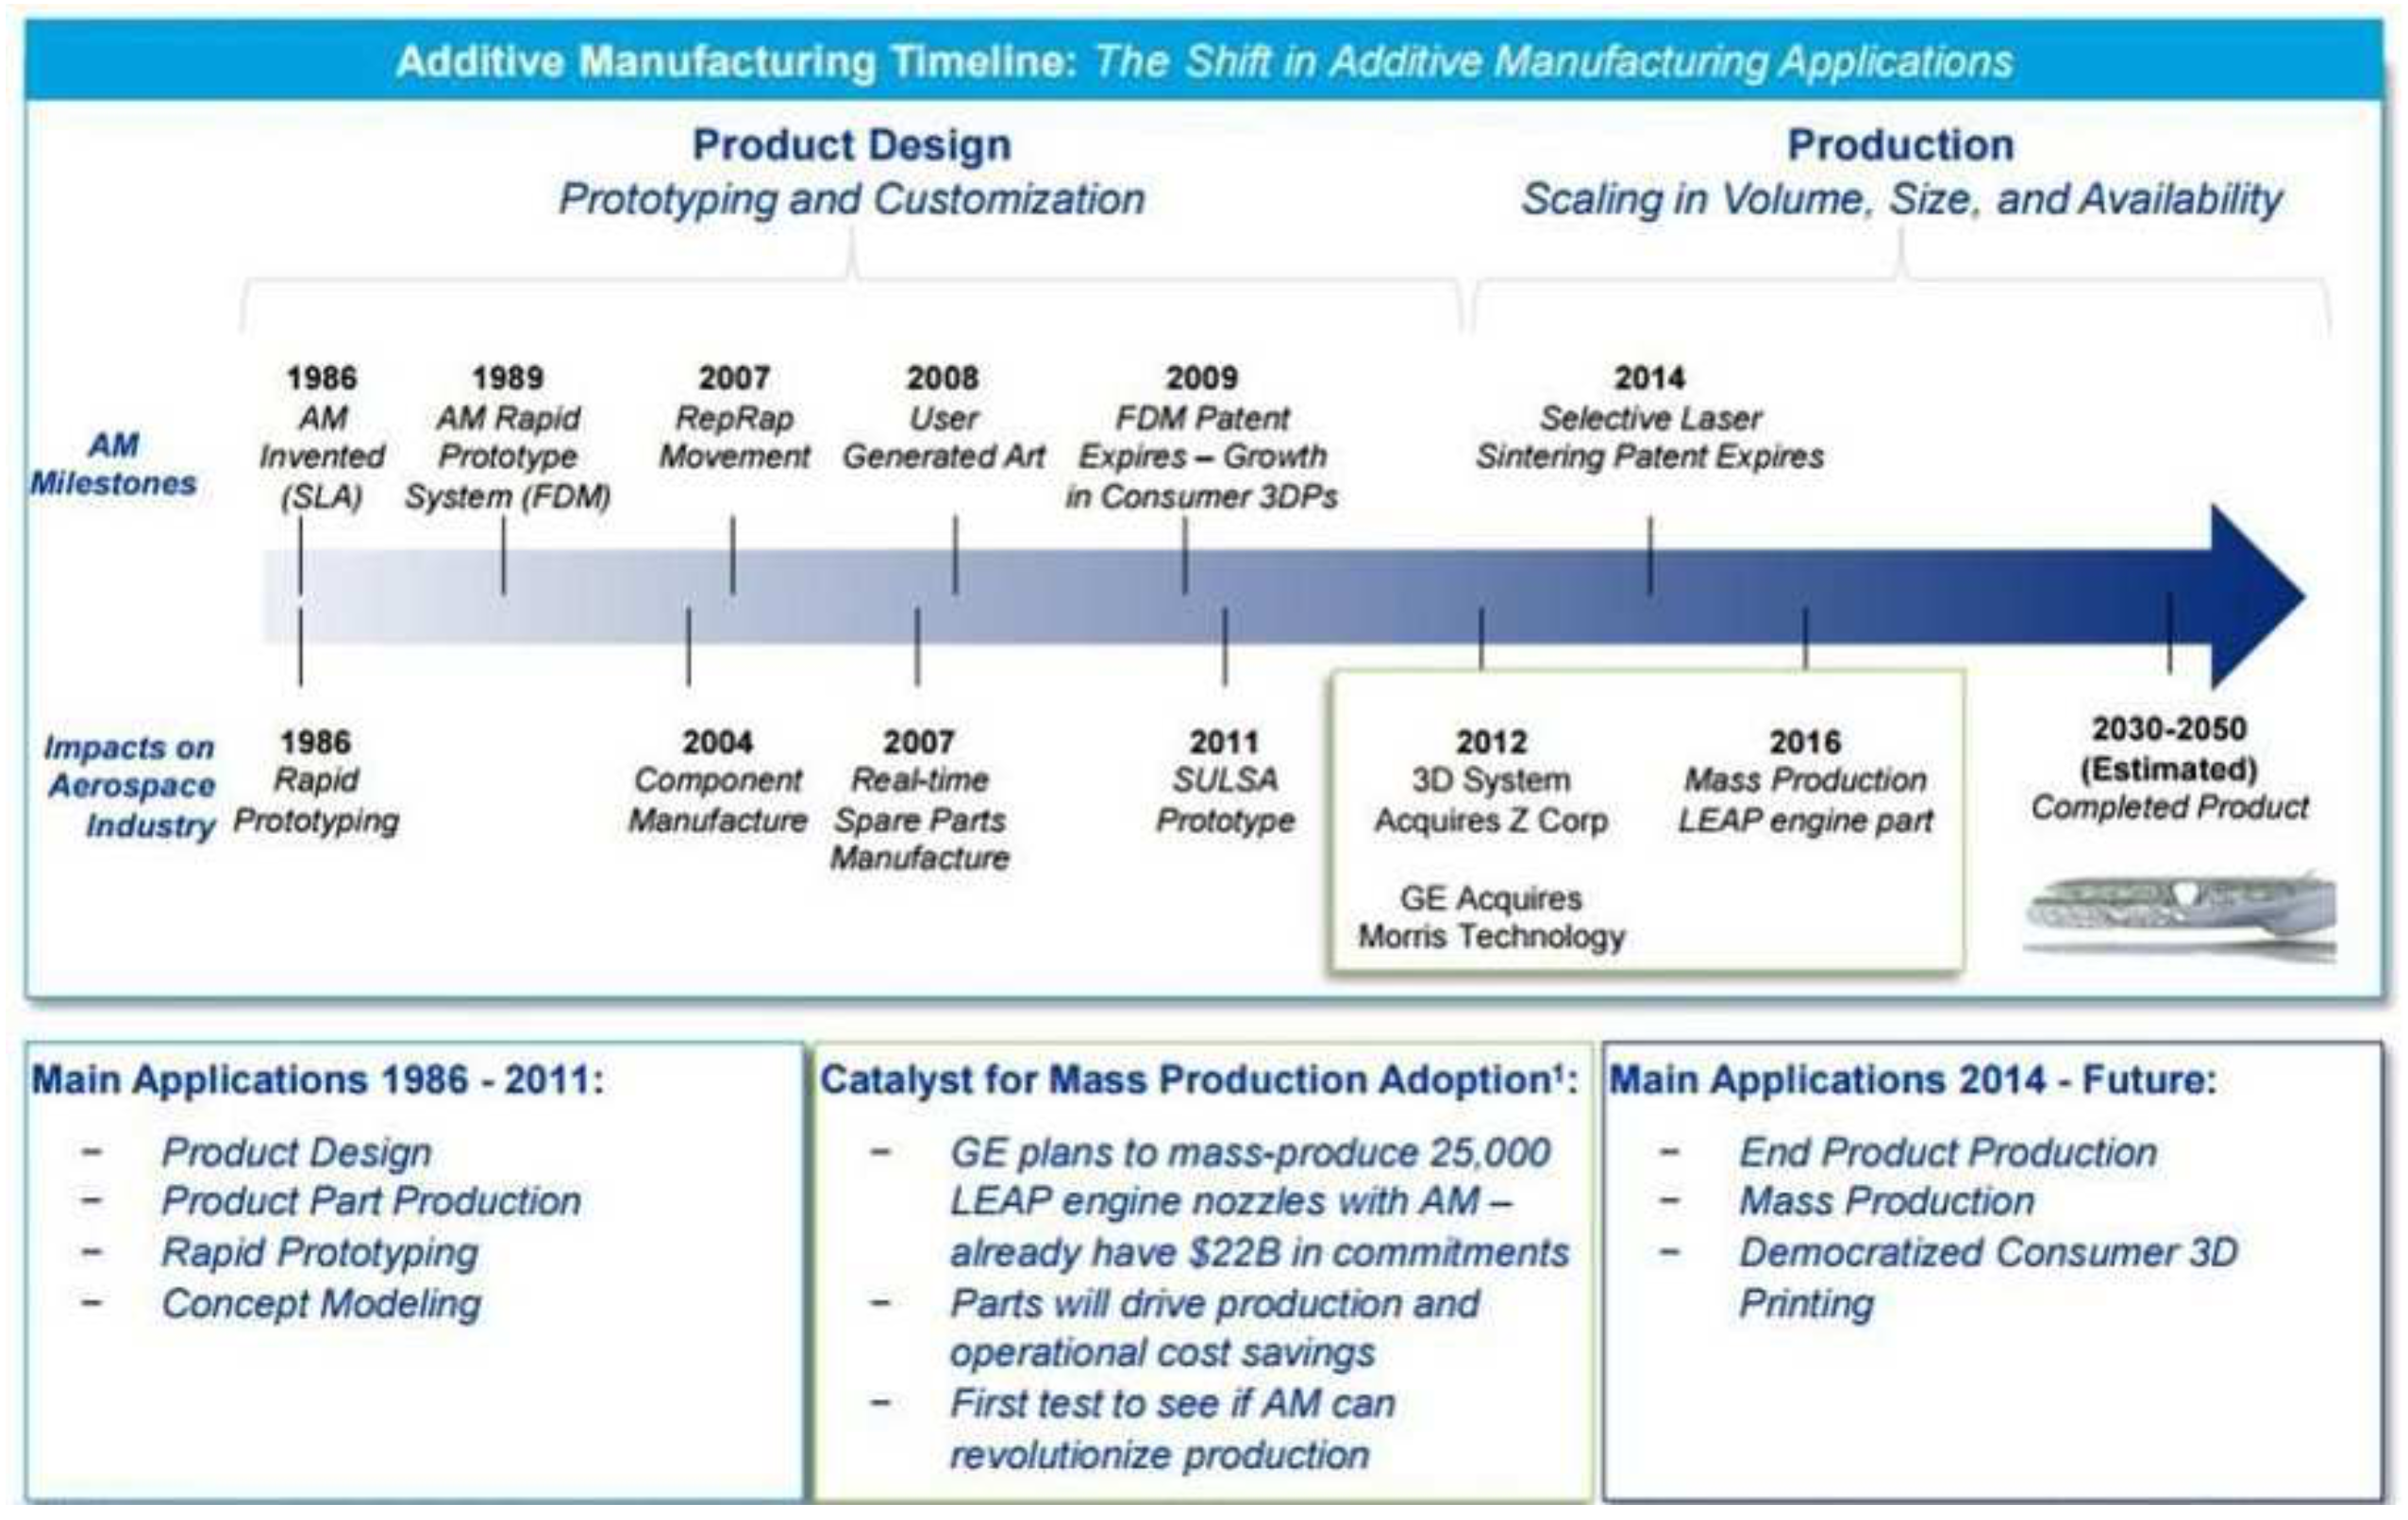
\includegraphics[width=0.8\textwidth]{./Images/AM_HISTORY}
\caption{AM important milestones}
\caption*{
\textbf{Source:} Additive manufacturing paths to performance, innova-tion, and growth\cite{cotteleer20143d}}
\label{AMHist}
\end{figure}
Additive manufacturing is defined as "the process of joining materials to make parts from 3D model data, usually by layer in combination with subtractive manufacturing"\cite{lee2017fundamentals}.
Over the years, AM has taken important steps, essentially in product design, as represented in the figure \ref{AMHist}.
The first steps of AM were in the 1980's, where parts called Rapid Prototyping were developed in a quick way to check their shape, fit and function\cite{bartolo2011history,bourell2016perspectives,wohlers2014history}.\par
In 1987, the company 3D systems developed a plastic processing system known as stereolithografy. This process consists of solidifying thin layers of polymer using a laser UV. Since then, many companies researched and made progresses in order to develop new technologies, improve process and commercialize them. \cite{bourell2016perspectives,wohlers2014history}\par
In the 90's, the bet of several companies allowed the development of other techniques based on polymers such as, \ac{FDM}, \ac{SGC},  \ac{LOM} and  \ac{SLS}.\cite{bourell2016perspectives,wohlers2014history}\par
In addition to the new AM techniques, processes based on Metals were initially introduced through laser sintering and only later by powder sintering.\cite{bourell2016perspectives,wohlers2014history}\par

The improvement of computers, CAD software also had a development that came to revolutionize the process, causing AM to take off exponentially in the mid 2000's. The internet had a strong influence on this growth by promoting global interaction.\cite{wohlers2014history}\par
Until the mid-2000's, AM was only possible as plastic softs as the prototyping goal. Since then, with the range of materials increasing sharply, it is possible to create new parts, strongers with more details and more functional characteristics.\cite{wohlers2014history}\par
The manufactured process is currently applied to almost all market areas, from electronics, aerospace and automobiles to education and medicine.
In the aerospace industry, AM has the potential to change the future of aircraft manufacturing, from design to construction.\par
The main aircraft manufacturers are already producing parts with AM although they are still non-critical parts and to a limited extention.\par 
Aircraft manufacturers strive to reduce the weight of aircraft and the use of AM can assist in this weight reduction \cite{birtchnell2013freight}.\par
Airbus has already adopted this technology. It changed internal components like brackets or cable routing cards from a conventional manufacturing process to 3D printing on its A350 \cite{warwick20153}.\par
Boeing applied 3D thermoplastic printing for prototypes and components for use on its 737,747,777 and 787 aircraft.\cite{walton20146th}
Some authors believe that the results of AM in this industry are livable and that in the near future we can have an aircraft almost 100\% manufactured with AM \cite{walton20146th}\cite{coykendall20143d}. However, not everyone agrees that AM will be able to overcome the efficiency and agility of the global freight industry.\par


\subsection{AM Processing Steps}

AM requires some steps of multiple difficulties depending on piece's complexity.\par
The process begins with the creation of a CAD model using a computer software or scanning an existing object. The software slices the CAD and creates a file with instructions for the machine.The machine creates the object layer by layer by forming each layer via the selective placement.After the Build Process is completed, the object is carefully cleaned and it may have to go through finishing processes, \textit{c.f.} figure \ref{Aviao}.\par

\begin{figure}[h]
\centering
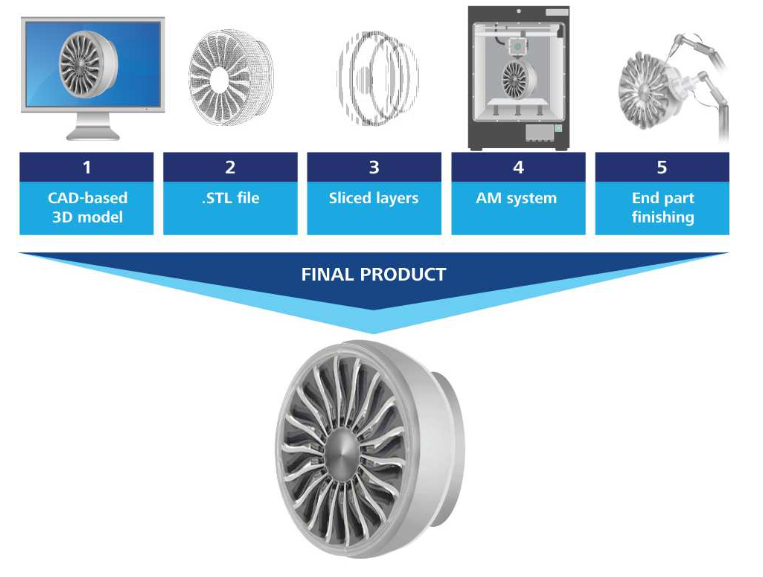
\includegraphics[width=0.5\textwidth]{./Images/AM_STEPS.png}
\caption{Generalized AM process}
\label{Aviao}
\caption*{\textbf{Source:}Cost estimation model for the directed energy deposition process adopting an activity-based approach \cite{santos2018cost}}
\end{figure}


\subsubsection{Modelling}
The\ac{AM} process must start with a 3D model using CAD software that must contain a precise internal and external description of the object.
This file will have to be converted to a language compatible with AM machines \cite{gibson2014additive}.\par
There are several file formats, the most used are \ac{STL} and \ac{AMF}.
STL transforms a simple model like a square box, where its surfaces can be approximated with twelve triangles. The most complex is the surface, the more triangles are produced. While the \ac{AMF} is a file format that allows for more details such as colors, materials and constellations\cite{gibson2014additive}.
Finally, with the specialized software's help, the file is divided into several transversal layers creating a new STI file, as shown in the figure \ref{STL}\cite{gibson2014additive}.
In this last point, there are some aspects to be considered such as the orientation of the piece, supports and support structure.

\begin{figure}[h]
\centering
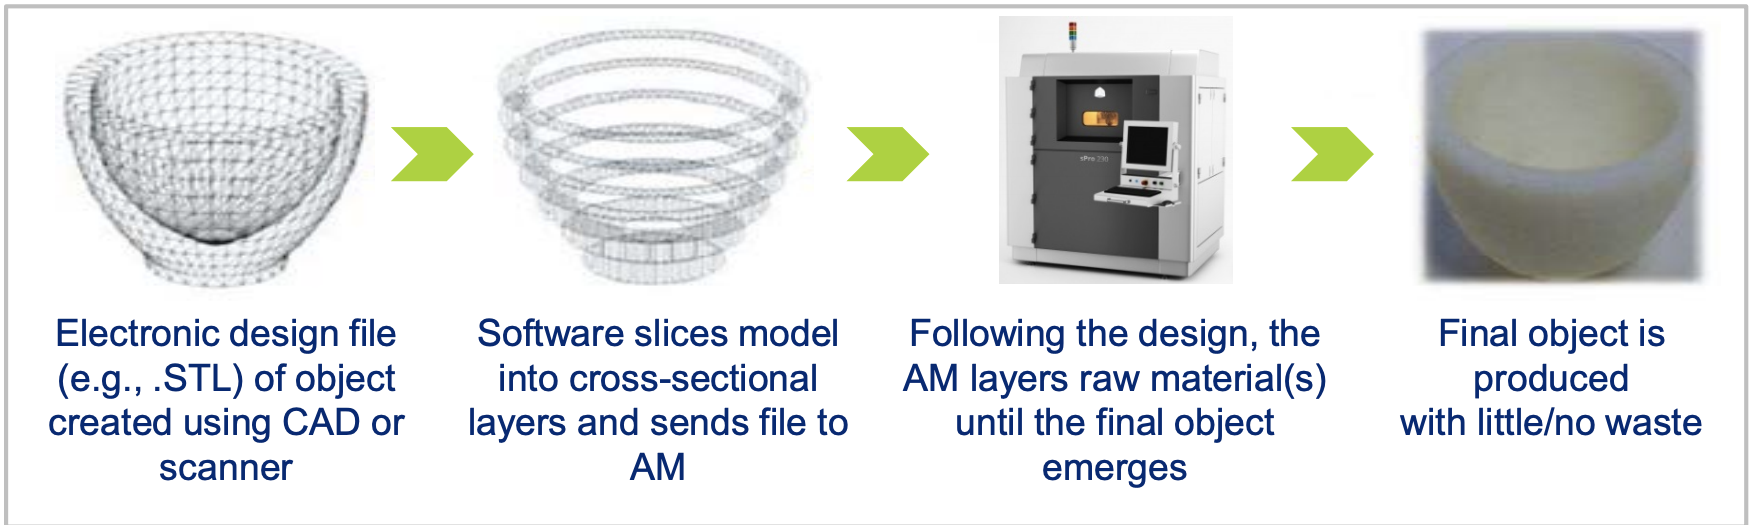
\includegraphics[width=0.5\textwidth]{./Images/STL.png}
\caption{Modelling Stages}
\label{STL}
\caption*{\textbf{Source:}Additive manufacturing paths to performance, innovation, and growth \cite{cotteleer20143d}}
\end{figure}



\subsubsection{Additive Manufaturing technologies}

This is the main stage of the whole process, after the AM machine receives the file, the part can then be produced.\par
First, the operator must configure the machine by preparing the raw material and determine the process parameters. Then the part's construction is in charge of the AM machine, which is an automated task that requires only the operator's supervision.\par
Additive manufacturing is, as the name itself implies, the process that adds material during the production of a part. For which, different technologies are used and regarding the technologies applied to metal parts, we can classify them in 4 main categories: \ac{MJ}, \ac{BJ}, \ac{PBF} and \ac{DED}.

\vspace{10}

\textbf{\emph{Material Jetting}}\par
\vspace{10}

\ac{MJ} is a 3D printing process more like conventional 2D printers. In the \ac{MJ}, a print head distributes droplets of a photosensitive material that solidifies under ultraviolet light, forming a layer\cite{lboro}. The material used in this technology is thermoset photopolymers in liquid form, figure \ref{MJ}.\par
Steps of the \ac{MJ} printing process:
\begin{enumerate}
    \item The resin is heated to 30-60C to achieve an ideal viscosity\cite{3dhubs}.
    \item The print head travels on the platform and deposits droplets at designated locations\cite{3dhubs}.
    \item A UV light source fixed to the print head cures the deposited material, solidifying it. Thus, it gives rise to the first layer of the piece\cite{3dhubs}.
    \item After the construction of the first layer, the platform goes down one layer height and the process is repeated until the entire piece is completed\cite{3dhubs}.
\end{enumerate}
\ac{MJ} is classified as a technology capable of producing smooth parts with surfaces compared to injection molding, with a high dimensional precision (more or less 0.1\%)\cite{3dhubs,lboro}. However, MJ parts are mainly purchased for prototypes not issued due to their poor mechanical properties. MJ is an expensive technology making it unviable for some applications\cite{lboro,3dhubs}.

\begin{figure}[h]
\centering
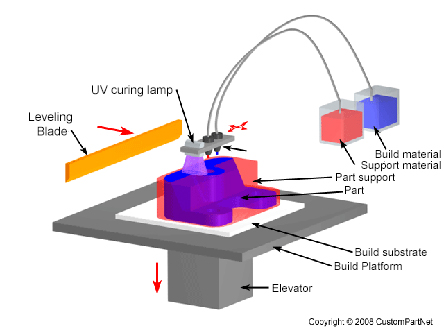
\includegraphics[width=0.6\textwidth]{./Images/MJ.jpg}
\caption{Material Jetting}
\label{MJ}
\caption*{\textbf{Source:} www.lboro.ac.uk}
\end{figure}
\\
\vspace{10}
\textbf{\emph{Binder Jetting}}\par
\vspace{10}
The Jet Binder is a multi-stage AM process developed by MIT in the early 1990s\cite{gokuldoss2017additive}.
This 3D printing process uses a powder-based material and a binder. An impression involves several processes:
\begin{enumerate}
    \item The powder material is spread on the construction platform using a roller \cite{lboro2}.
    \item The print head deposits the bonding adhesive on the powder, when necessary \cite{lboro2}.
    \item The construction platform is lowered by the layer thickness of the model \cite{lboro2}.
    \item Another layer of dust is spread over the previous layer. The object is formed where the powder binds to the liquid \cite{lboro2}.
    \item Dust not attached to the position around the object \cite{lboro2}.
    \item The process is repeated until the entire object is made\cite{lboro2}.
\end{enumerate}

\ac{BJ} allows a wide variety of colors and allows the use of raw materials such as metals, polymers and ceramics.
However, due to the use of binder, the parts are not suitable for structural parts. \cite{ziaee2019binder,gokuldoss2017additive}.

\begin{figure}[h]
\centering
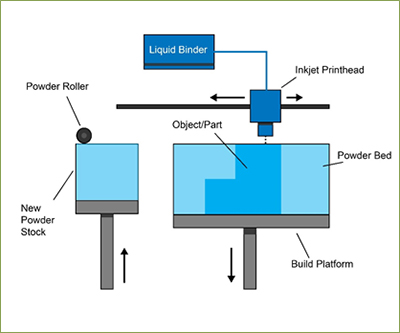
\includegraphics[width=0.4\textwidth]{./Images/BinderJet.jpg}
\caption{Binder Jet\\
Source: https://www.lboro.ac.uk/}
\label{}
\end{figure}

\vspace{50}
\textbf{\emph{Powder Bed Fusion}}\\
\vspace{5}
\ac{PBF} methods use an electro or laser beam to melt and melt the metal powder.In the figure \ref{PBF} we can see a schematic of a \ac{PBF} machine. Building a part with \ac{PBF} has the following steps:
\begin{enumerate}
    \item A layer of metallic powder is spread on the platform.
    \item A laser melts the first layer
    \item A new layer of powder is spread on the previous layer using a roller.
    \item More layers are spread, fused and added
    \item The process is repeated until the entire model is created.
\end{enumerate}

This process has several techniques for melting metal powder such as: DMLS, EDM, SHS, SLM and SLS.\par

DMLS, was developed by Germany's EOS. This printing technique fuses very thin layers of metallic powder using a yb fiber laser beam. The system operates in a protective atmosphere of nitrogen and argon allowing the use of a wide range of metals. \cite{udroiu2012powder}\par
DMLS has an excellent and precise resolution in the creation of its objects, being used for the construction of prototypes of instruments, instruments and objects for the use of the aeronautical and space industry. \cite{3dilla}\par
EDM developed by the Swedish company Arcam, builds the pieces layer by layer by melting the metallic powder through an electron beam. When electrons reach the metallic powder at high speed, the kinetic energy is converted into thermal energy by melting the metallic powder. \cite{udroiu2012powder}\par
The high quality of finish allows this process to become standard for medical applications and parts construction for aircraft \cite{lboropbf}.
SHS uses a heated thermal printing head to melt the powder material. The use of this thermal head and not a laser permanent the necessary electrical energy. The process is used for prototypes not to use. \cite{lboropbf}\par

SLM uses a high-power iterbium fiber laser to fuse or metallic powder\cite{udroiu2012powder}.  A roller or blade is used to spread the powder, which is then melted by the laser, building the piece in layers. It is a relatively fast process that requires the use of an inert gas and has high energy costs \cite{lboropbf}.\par
This technique is used for dental application, turbine blade with internal shaped cooling channels, vane segment for aerospace applications. \cite{udroiu2012powder}\par
SLS and SLM have the same principle, differing only in that the SLM achieves a complete fusion of the powder layers and the SLS does not \cite{wagner2016additive}. The SLS process benefits from having no additional support structure and from some machines monitoring the temperature of layers by automatically adapting the laser power. The models have a cooling period to guarantee a high tolerance and quality of fusion. \cite{lboropbf}
\begin{figure}[h]
\centering
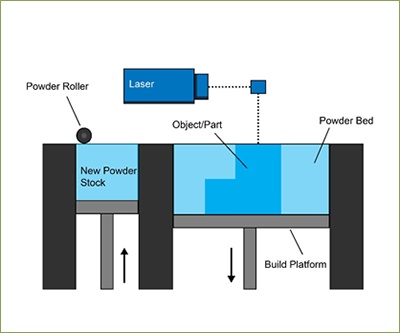
\includegraphics[width=0.4\textwidth]{./Images/PBF.jpg}
\caption{Powder Bed Fusion Machine}
\label{PBF}
\caption*{\textbf{Source:} www.lboro.ac.uk}
\end{figure}
\\

\\ \textbf{\emph{Directed Energy Deposition}}\\
\par
DED is a collection of processes that uses thermal energy, laser or electron beam, focused on melting and bonding materials in the form of powder or wire\cite{shamsaei2015overview}.\par
The process can be used with polymers, ceramics but it is with metals that DED together with GMP, are more reliable and used AM techniques.
Almost all weldable metals can be printed with DED. This includes titanium and its alloys, inconel, tantelo, aluminum, etc\cite{bourell2017materials,shamsaei2015overview}.\par
A typical DED machine consists of a nozzle mounted on a multi-axis arm, which moves in 4 or 5 directions, which deposits the material by melting on the specific surface where it solidifies. \par
DED consists in the following steps\cite{DED2}:
\begin{enumerate}
    \item The arm with the nozzle moves on the printing platform.
    \item The material is deposited by the spout on the platform's surface.
    \item The material is supplied in the form of wire or powder.
    \item The material is melted using a laser or electron source after deposition.
    \item More layers are added until the object is finished.
\end{enumerate}

DED presents itself as a fast and inexpensive AM technology compared to the others. However, fusion processes require more research and improvement of fusion processes and require post-processing to achieve the desired effect\cite{DED}.

\begin{figure}[h]
\centering
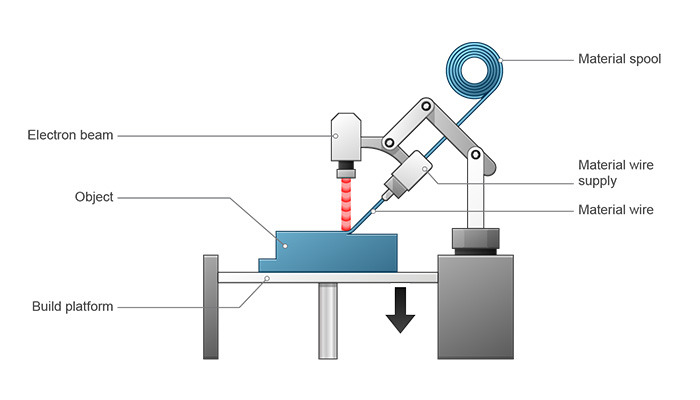
\includegraphics[width=0.6\textwidth]{./Images/DED.jpg}
\caption{DED\\
Source: \cite{DED2}}
\label{DED}
\end{figure}
\\

\subsubsection{Finishing Process}
 
 \textbf{\emph{ Shot Peening}}\\

 
 Shot peening is a cold working process used in the aerospace and automotive industries \cite{meo2003finite}.\par
Surface treatment procedures such as grinding, milling, bending or heat treatment procedures cause residual tensile stress. This Residual Tensile Effort leads to a reduction in the life cycles of the parts. Shotpeening converts Residual Tensile Stress into Residual Compression Stress, which allows to increase the complication of the service life and as maximum load resources of the parts.\cite{majzoobi2005three}\par

The process is used for better resist once to metals' fatigue. It consists of bombarding small hardened spheres, usually steel, against a surface of the object creating small plastic deformations on the part's surface, causing changes in the mechanical properties. \cite{majzoobi2005three,meo2003finite}\par
The impact of each shot particle on the object generates a compression stress on the surface of the piece. A surface notched by the ball generates a compaction force below the notch. Hammering generates not only one but severals notches on the surface, forming a layer of residual compaction stress on the part. \cite{meo2003finite,SP}\par
The creation of the residual compression stress created on the part's surface helps to prevent the appearance of cracks as they cannot propagate in the compression environment generated by hammering. \cite{meo2003finite,SP}\par

\begin{figure}[h]
  \centering
  \begin{minipage}[b]{0.4\textwidth}
    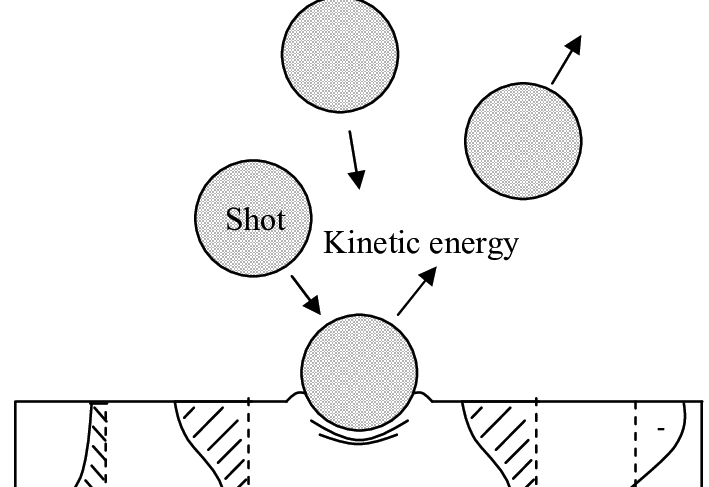
\includegraphics[width=\textwidth]{./Images/sp1.png}
    \caption{Compression Stress}
    \label{grinder1}
    \caption*{\textbf{Source:} Texture Gradients in Shot Peened \cite{maawad2010texture}}
  \end{minipage}
  \hfill
  \begin{minipage}[b]{0.4\textwidth}
    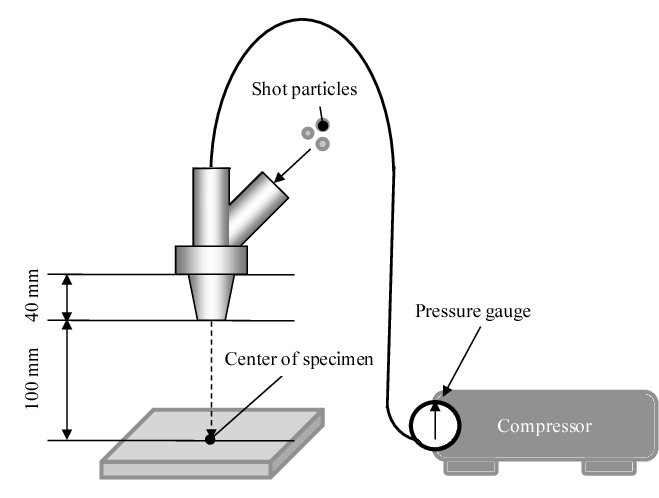
\includegraphics[width=\textwidth]{./Images/sp.png}
    \caption{Shot Peening Machine}
    \label{grinder2}
    \caption*{\textbf{Source:} Modelling  of  particle  behaviour  in  shot  peening  process \cite{kato2014modelling}}
  \end{minipage}
\end{figure}

\vspace{20}
 \textbf{\emph{Hot Isostatic Pressing}}\\


\ac{HIP} is a post processing used to reduce porosity of metals and increase the density of ceramic materials.
The process consists of placing the object in a chamber where it is pressed on all sides with equal pressure (isostatic pressure) and with an elevated temperature for consolidation in a dense solid\cite{atkinson2000fundamental}. \ac{HIP} applies high temperatures from several hundred to 2000\degree C and isostatic pressure from several tens to 200MPa at the same time. Argon gas is the most used pressure medium. The gas at 1000\degree C and under pressure 98MPa can cause an intense convection due to the low density, viscosity coe and high thermal expansion coe\cite{HIP}.\par
Through \ac{HIP} it is possible to obtain material formats not very different from the initial one after high pressures, contrary to what happens with hot press, see in the figure\ref{hip1}\ref{hip2}. \cite{atkinson2000fundamental}.
\ac{HIP} is used in a wide range of fields:
\begin{itemize}
    \item Pressure powder sintering;
    \item Diffusion connection of different types of materials;
    \item Removal of residual pores in sintered items;
    \item Removing internal defects in castings;
    \item Rejuvenation of parts damaged by fatigue or creep;
    \item High pressure impregnated carbonization method.
\end{itemize}




\begin{figure}[h]
  \centering
  \begin{minipage}[b]{0.3\textwidth}
    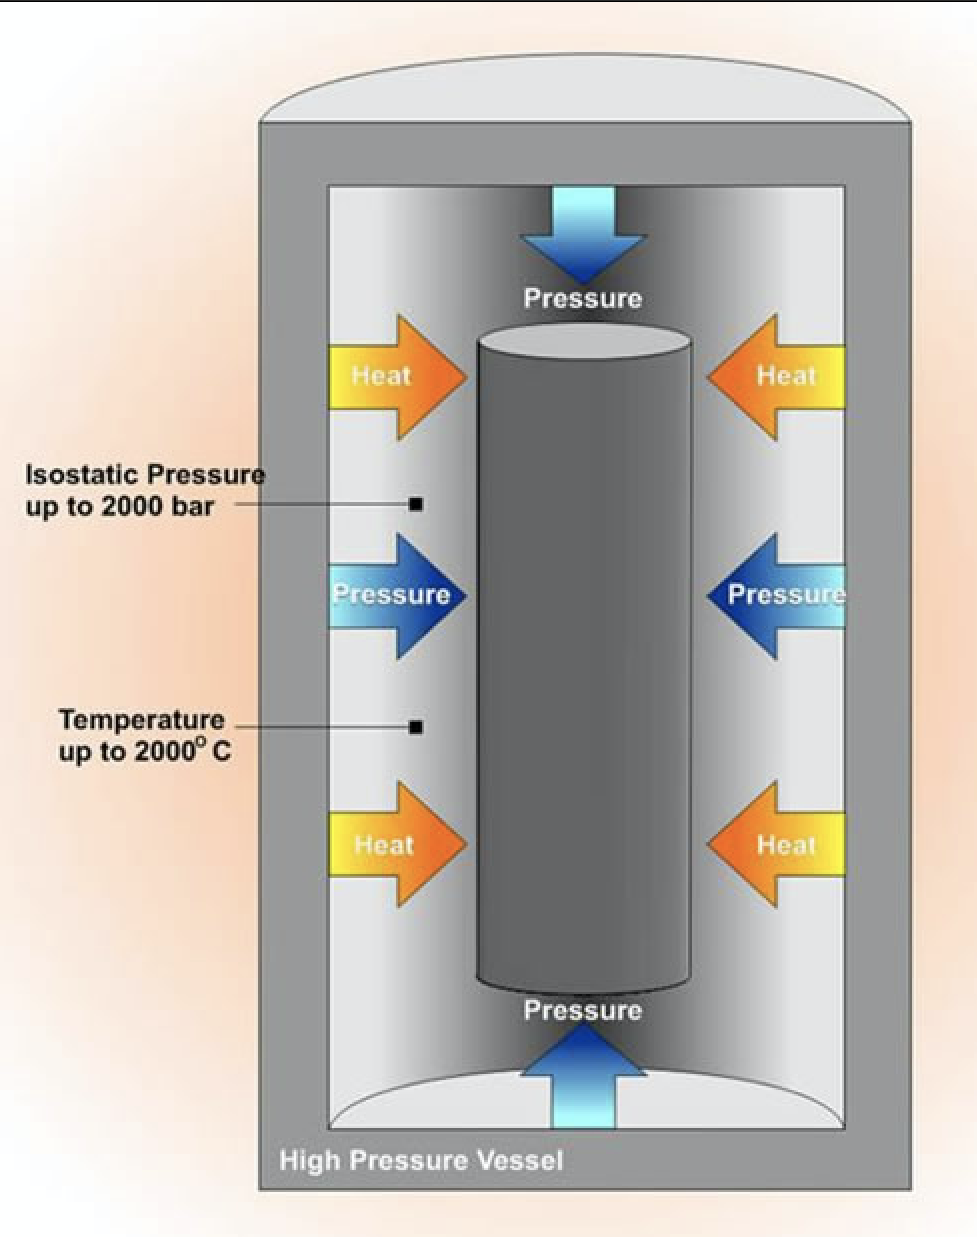
\includegraphics[width=\textwidth]{./Images/hp1.png}
    \caption{HIP process}
    \label{hip1}
    \caption*{\textbf{Source:} www.azom.com}
  \end{minipage}
  \hfill
  \begin{minipage}[b]{0.5\textwidth}
    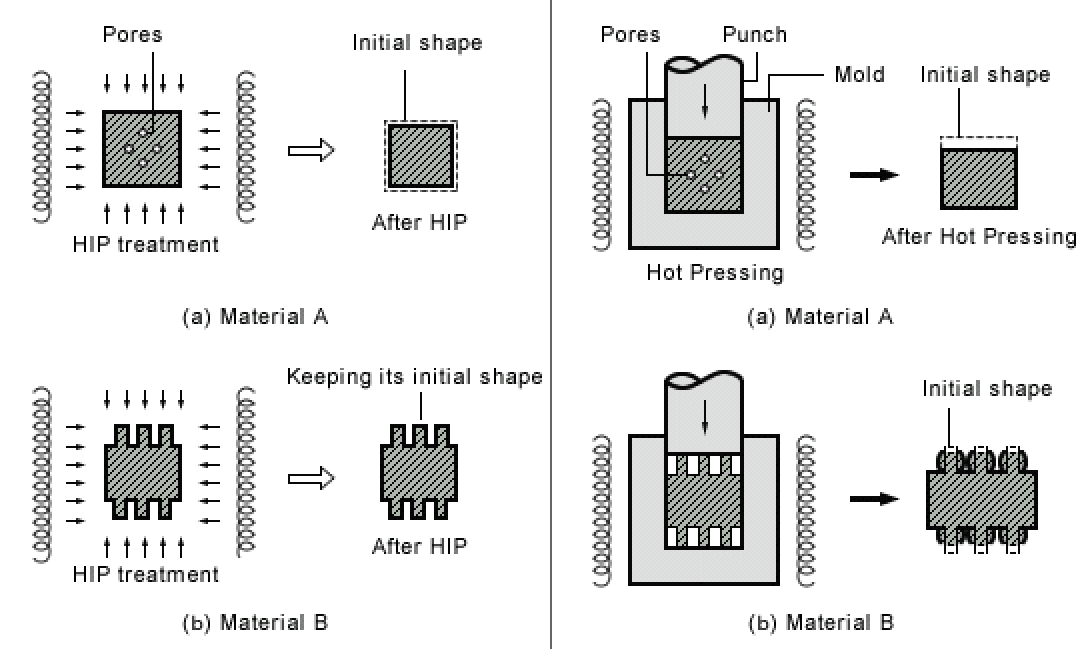
\includegraphics[width=\textwidth]{./Images/hp2.png}
    \caption{HIP vs conventional compression}
    \label{hip2}
        \caption*{\textbf{Source:} www.kobelco.co.jp}
  \end{minipage}
\end{figure}



\section{Capabilities and Challenges of Additive Manufacturing and Forging}

Additive Manufacturing is widely adopted in many industrial sectors, particularly in the aeronautical sector. The main companies in the world are converting to this technology but not leaving the forging part in the production of their parts. It is important to note the main differences and limitations of the technologies:\\
\vspace{20}\\
 \textbf{\emph{Strengh}}: Although \ac{AM} already works with a wide variety of raw materials, its results still have a high degree of uncertainty. Therefore, its use is limited to parts that provide little mechanical effort, since deposited layers can create weakened parts if they are not perfectly calibrated\cite{AMD}. The total density of AM metal parts is not possible without the subsequent \ac{HIP}. On the other hand, forging is a well-known technique, widely used and reliable, with the properties of the materials already tabulated. Deposited layers can create weakened parts if they are not calibrated perfectly
 \vspace{20} \\
 \textbf{\emph{Design Complexity}}: Parts with more complex geometries and internal cavities are a limitation of conventional forging. With conventional techniques it is difficult to produce objects with a high complexity and detail and sometimes they have to be subdivided into several less complex parts, which subsequently without connections forming an original piece\cite{he2007transport}.
With the tools of advanced software and AM brought the possibility to produce uniform parts with complex changes geometries and high internal and external resolution\cite{toyserkani2004laser}.
 \vspace{20}\\
 \textbf{\emph{Part Size }}: AM has restrictions on the size of the parts. The size of the objects is limited to the size of the machine's printing chamber. Producing large chambers for AM machines is expensive, since inert atmospheres or vacuums are required. On the other hand, AM allows you to produce very small parts with high detail\cite{saboori2017overview}.
With forging there is no limitation on the parts's size, it is necessary to adapt only the size and strength of the hammers and presses, as well as the EDM and Multi Axis Mills cutting machines. Compared to the production of micro parts, they lose detail as they become smaller\cite{saboori2017overview}\cite{frazier2014metal}.
 \vspace{20}\\
  \textbf{\emph{Timings}}: The 3D impression of a product compared to forging has a significant reduction in time if we think about all stages of production. Engineers can create a prototype with AM immediately after its design - so you can be tested as its properties and not wait weeks or months for a traditionally manufactured prototype to arrive.\cite{AMPC}\par
  On the other hand, for higher production volumes, conventional manufacturing mechanisms are still the fastest choice, at least until AM printers become better and faster.
 \cite{attaran2017rise}
  
 \vspace{20}\\
 \textbf{\emph{Weight Parts}}: AM it became possible to produce weight with complex structures compared to forging without compromising some of its properties. What becomes a great advantage for some industrial sectors like an Aerospace that looks for the lightest parts to improve fuel efficiency \cite{huang2016energy}.
 \vspace{20}\\


 \textbf{\emph{Tooling}}: The comparison of 3D printing for the traditional manufacture of electronic components, researched in Italy found out that 93.5\% of the cost of manufacturing a product using the traditional method is linked to tools. \cite{boubekri2015economics}
A strong advantage of additive manufacturing is the ability to significantly reduce or eliminate the use of tools.
 \vspace{20}\\
 \textbf{\emph{Material Waste}}: Traditional methods such as forging generate a significant amount of waste. However, with AM, only the amount of raw material needed to produce a product is used.
Thus reducing waste with 3D printing will also have a positive impact on the environment. \cite{boubekri2015economics}
 \vspace{20}\\
 \textbf{\emph{Manufacturing}}:
In a conventional metohd the production of the pieces is done in several places and then stored, after which they can be distributed when necessary. With AM, parts are produced simultaneously in the same production and in the same place. It allows the possibility of reducing inventories, as it is possible to produce parts in remote locations on demand, eliminating large warehouses of stocks and the need for transportation \cite{tofail2018additive}\cite{pereira2019comparison}.
 \vspace{20}\\
 \textbf{\emph{Cost Prodution}}: 3D printing offers a good solution for manufacturing small quantities. Forging requires a large investment in die and custom tools not being economically profitable for low demands \cite{boubekri2015economics}.
On the other hand, additive manufacturing does not offer economies of scale. \cite{boubekri2015economics}
 \vspace{20}\\
 \textbf{\emph{Produts Quality }}:AM technologies still have some quality limitations in terms of tensile stresses and in terms of construction resolution in same technology cases, with significant surface roughness. In contrast, forging is a much more studied method with reliable and known results\cite{tofail2018additive}.
 \vspace{20}\\
  \textbf{\emph{Finishing Equipment}}: The parts produced with AM when compared with the parts produced with conventional method have greater roughness and purity, forcing the post-processing \cite{AMD}. To eliminate the roughness characteristic of AM technology, surface treatment using the grinder or shot peening is necessary. For parts produced using powder, they have purity that will have to be treated with a hot isostatic press that will reduce the purity and increase the part's resistance \cite{loh1992overview}. Particularity of \ac{PBF}, is the use of supports in printing that after printing have to be separated from the part that can be removed with a water bath if they are soluble or cut using cutting tools if they are insoluble in water.\par
 \vspace{20}
 
 \noindent
  \textbf{\emph{Raw Materials}} - Currently, additively manufactured parts still have little variety of materials available. Despite the constant innovation and research in this new technology, the truth is that the raw materials associated with it are still scarce \cite{herzog2016additive}. Forging on the other hand has a greater variety of raw materials available.\par
 

\newpage
\section{Costs Modelling}
 
 \vspace{20}\\

Over the years, mass production factories have been migrating to developing countries such as China and India. Large American and European companies have been forced to rapidly shift production to lower volumes of innovative and sustainable products with high added value. Due to the need of greater flexibility and low-cost volume production, manufacturers have been looking for tools and new techniques. One of the emerging techniques is additive manufacturing. AM allows for freedom of design, removal of tool requirements and good profitability for low economic volumes. \cite{mellor2014additive}\par
Comparison conventional manufacturing methods with AM has been a constant issue on companies and production engineers. 3D printing of metallic hair combined with the part's redesign has a positive impact on cost savings. \cite{atzeni2012economics}\par
There are three ways to assess the costs of additive manufacturing:
\begin{itemize}
    \item The first is to study under what circumstances AM is competitive in relation to traditional methods \cite{thomas2014costs}. In this analysis, it is not only important to assess the production costs of the part but also the economic impact that the part will have in all of its life cycle. For example, a part adapted with additive manufacture that at the outset its production is more expensive than the same part by a traditional method, can be profitable in the long run, if it has a weight reduction of 18\% which will allow a savings aircraft fuel tank.  
    \item A second approach is to study all stages of production in additive manufacturing. This approach aims to estimate the cost of each process's stage, identify when and where resources are being consumed and whether there may be a reduction in the use of these resources \cite{thomas2014costs}.
    \item A third approach is to compare different additive manufacturing technologies. It's importante to know which are the most profitable for each situation, not only in the printing of the same but also in its post processing. However, despite the growth of this technology, purchase with conventional manufacturing methods has been scarce.
\end{itemize}




The first development work entirely to assess the cost of\ac{AM} was launched in 2003 by Hopkinson and Dickens \cite{hopkinson2003analysis}. The authors calculated the cost of producing an integrated part by additive manufacturing based on 3 premises\cite{costabile2017cost}:
\begin{enumerate}
    \item the system produces a single kind of play for a year 
    \item uses maximum volumes 
    \item the machine operates 90\% of the time.  
\end{enumerate}


In this model, costs can be divided by machine, labor and material costs, with energy and building costs being practically neglected with only 1\% of total costs. \cite{thomas2014costs,costabile2017cost}
The authors report the cost estimate using the traditional injection model method with \ac{LS}, \ac{FDM} and \ac{LS} in terms of costs by various quantities.\par 
\ac{LS} manufacture was compared against \ac{IM} techniques in order to find when \ac{RM} was economically, figure \ref{HD}. 
\begin{figure}[h]
\centering
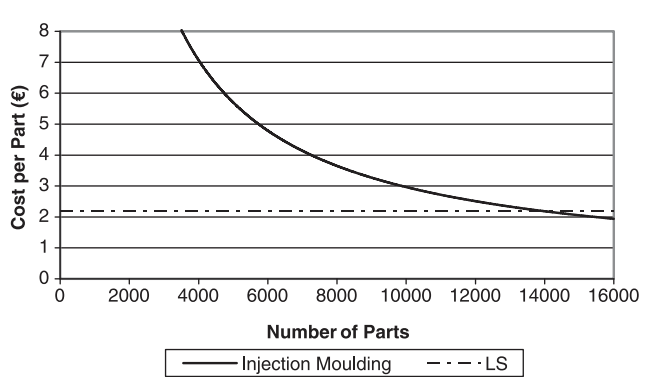
\includegraphics[width=0.6\textwidth]{./Images/HD.png}
\caption{Example of break-even analysis comparing LS with
IM}
\label{HD}
\caption*{\textbf{Source:} Cost estimation for rapid manufacturing ’ simultaneous production of mixed components using laser sintering \cite{ruffo2007cost}}
\end{figure}
\\
This model is a good approximation, but only validated when:
\begin{itemize}
    \item high production volumes
    \item production of the same piece
\end{itemize}

Later, in 2006, Ruffos \cite{ruffo2006cost}, a study based on the total cost, dividing them into labor, material, energy, administration and general costs.\cite{thomas2014costs,ruffo2007cost}\par
In contrast to the previous cost, developed by Hopkinson and Dickens, Ruffos' cost model has a curve that relates the cost per part to the volume of production and has the shape of a sawtooth. \cite{ruffo2007cost}\ref{Ruffos} \par
The Hopkinson and Dickens model was compared with that of Ruffos, now a comparison of evidence is an underestimation of the Hopkinson and Dickens model.\cite{thomas2014costs,ruffo2007cost}\par

\begin{figure}[h]
\centering
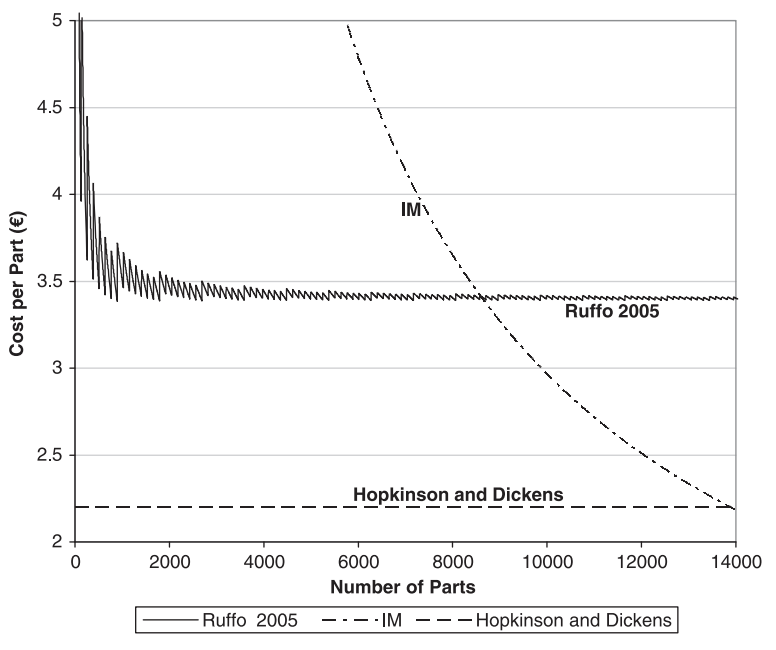
\includegraphics[width=0.5\textwidth]{./Images/3models.png}
\caption{Cost model comparison of \ac{LS} and \ac{IM}}
\label{Ruffos}
\caption*{\textbf{Source:} Cost estimation for rapid manufacturing ’ simultaneous production of mixed components using laser sintering \cite{ruffo2007cost}}
\end{figure}

Hopkinson, Dickens and Ruffos were the first to develop cost estimates for additive manufacturing. However, both authors developed models where they did not take into account the post processing of the parts, only the manufacture of the part.\par
Over the past decade, more complete new models have been developed. We can find quite complete models for certain production steps or for a specific production line.\par

Each piece has a set of production steps depending on its purpose and on the method used for its construction. A part produced with forging does not have the same post-processing as a part produced by \ac{AM}. Like a structural part, it does not have the same post-processing as a prototype. In this way, a flexible model is required where the editing of the production line of that particular part is allowed.\par
Therefore, the development of a cost model where the stages of manufacture can be selected is an important goal that has not been achieved and this is a gap extremelly important to fill in.

